\documentclass[11pt, letterpaper]{article}

% Fonts and Encoding
\usepackage[utf8]{inputenc}
\usepackage[T1]{fontenc}
\usepackage{lmodern} % High-quality Latin Modern vector font

% Math and Symbols
\usepackage{amsmath, amssymb, amsthm, amsfonts, mathrsfs, mathtools}

% Layout and Geometry
\usepackage{geometry}
\geometry{letterpaper, margin=1in}
\setlength{\parindent}{0pt}
\setlength{\parskip}{0.6em}

% Formatting and Graphics
\usepackage{graphicx, xcolor, enumitem, booktabs, array, tabularx}

% TikZ for Illustrations
\usepackage{tikz}
\usetikzlibrary{arrows.meta, positioning, shapes.geometric, calc, backgrounds, matrix}

% Clickable Links and TOC
\usepackage{hyperref}
\hypersetup{
    colorlinks=true,
    linkcolor=blue,
    filecolor=magenta,      
    urlcolor=cyan,
    pdftitle={Solving Initial Value Problems with Laplace Transforms},
}

% Theorem Environments
\newtheorem{theorem}{Theorem}[section]
\newtheorem{lemma}[theorem]{Lemma}
\newtheorem{proposition}[theorem]{Proposition}
\newtheorem{corollary}[theorem]{Corollary}
\theoremstyle{definition}
\newtheorem{definition}{Definition}[section]
\newtheorem{axiom}{Axiom}[section]
\newtheorem{example}{Example}[section]
\theoremstyle{remark}
\newtheorem{remark}{Remark}[section]

% Custom Commands (Enforced standard notation)
\newcommand{\R}{\mathbb{R}}
\newcommand{\N}{\mathbb{N}}
\newcommand{\Z}{\mathbb{Z}}
\newcommand{\Q}{\mathbb{Q}}
\newcommand{\E}{\mathbb{E}}
\newcommand{\Prob}{\mathbb{P}}
\newcommand{\F}{\mathcal{F}}
\newcommand{\Lap}{\mathcal{L}}

\title{Solving Initial Value Problems with Laplace Transforms}
\author{Tashfeen Omran}
\date{\today}

\begin{document}

\maketitle
\tableofcontents
\newpage

\section{Part 1: Comprehensive Introduction, Context, and Prerequisites}

\subsection{Core Concepts}
The Laplace transform is a powerful integral transform that maps a function of time, $f(t)$, into a function of a complex variable, $F(s)$. In the context of differential equations, its primary utility lies in its ability to convert linear ordinary differential equations (ODEs) into algebraic equations. 

When solving an Initial Value Problem (IVP), traditional methods require finding a general solution first and then applying initial conditions to solve for unknown constants. The Laplace transform method bypasses this entirely. By taking the transform of both sides of an ODE, the initial conditions are naturally embedded into the resulting algebraic equation. Solving for the transformed solution, $Y(s)$, and then applying the inverse Laplace transform, $\Lap^{-1}\{Y(s)\}$, yields the specific solution $y(t)$ directly.

\subsection{Intuition and Derivation}
The fundamental mechanism that makes the Laplace transform useful for ODEs is the \textit{Derivative Property}. Consider the definition of the Laplace transform:
\[ \Lap\{f(t)\} = \int_{0}^{\infty} e^{-st} f(t) \, dt \]
If we want to find the transform of a derivative, $f'(t)$, we use integration by parts:
\[ \Lap\{f'(t)\} = \int_{0}^{\infty} e^{-st} f'(t) \, dt \]
Let $u = e^{-st}$ and $dv = f'(t) \, dt$. Then $du = -s e^{-st} \, dt$ and $v = f(t)$.
\[ \Lap\{f'(t)\} = \left[ e^{-st} f(t) \right]_{0}^{\infty} - \int_{0}^{\infty} -s e^{-st} f(t) \, dt \]
Assuming $f(t)$ is of exponential order such that $\lim_{t \to \infty} e^{-st} f(t) = 0$, we get:
\[ \Lap\{f'(t)\} = -f(0) + s \int_{0}^{\infty} e^{-st} f(t) \, dt = sF(s) - f(0) \]
This derivation shows exactly why the initial condition $f(0)$ appears. The transform of a derivative in the time domain becomes multiplication by $s$ in the frequency domain, minus the initial state.

\subsection{Historical Context and Motivation}
The mathematical foundations of the transform were laid by Pierre-Simon Laplace in the late 18th century during his work on probability theory and celestial mechanics. However, it was the English electrical engineer Oliver Heaviside in the late 19th century who popularized operational calculus. Heaviside needed a robust mathematical framework to analyze complex electrical circuits with switches (discontinuous forcing functions). He treated the differential operator as an algebraic variable, a method that was initially criticized for lacking rigor but was later fully justified by the Laplace transform framework.

\subsection{Key Formulas}
\renewcommand{\arraystretch}{1.5}
\begin{tabularx}{\textwidth}{X >{$\displaystyle}c<{$}}
\toprule
\textbf{Description} & \textbf{Formula} \\
\midrule
Transform of First Derivative & \Lap\{y'\} = sY(s) - y(0) \\ \relax
Transform of Second Derivative & \Lap\{y''\} = s^2Y(s) - sy(0) - y'(0) \\ \relax
Transform of Third Derivative & \Lap\{y'''\} = s^3Y(s) - s^2y(0) - sy'(0) - y''(0) \\ \relax
Multiplication by $t^n$ & \Lap\{t^n f(t)\} = (-1)^n \frac{d^n}{ds^n} F(s) \\ \relax
First Shifting Theorem & \Lap\{e^{at} f(t)\} = F(s - a) \\
\bottomrule
\end{tabularx}

\subsection{Prerequisites}
To successfully navigate this topic, you must be proficient in:
\begin{itemize}
    \item \textbf{Partial Fraction Decomposition (PFD):} Breaking down complex rational functions into simpler fractions (including handling repeated roots and irreducible quadratics).
    \item \textbf{Completing the Square:} Essential for matching irreducible quadratic denominators to sine and cosine transform templates.
    \item \textbf{Basic Integration:} Specifically, solving first-order linear ODEs using integrating factors, which is required when the original ODE has variable coefficients (like $t y''$).
\end{itemize}

\begin{center}
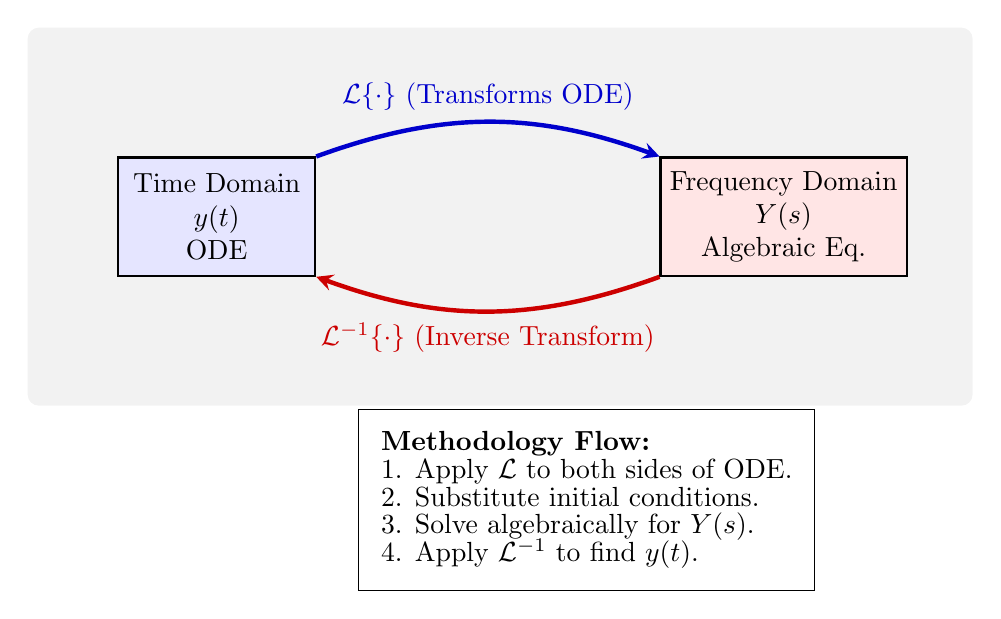
\begin{tikzpicture}[scale=1.2]
    % Background
    \fill[gray!10, rounded corners] (-1, -2) rectangle (9, 2);
    
    % Nodes
    \node[draw, thick, fill=blue!10, minimum width=2.5cm, minimum height=1.5cm, align=center] (time) at (1, 0) {Time Domain \\ $y(t)$ \\ ODE};
    \node[draw, thick, fill=red!10, minimum width=2.5cm, minimum height=1.5cm, align=center] (freq) at (7, 0) {Frequency Domain \\ $Y(s)$ \\ Algebraic Eq.};
    
    % Arrows
    \draw[->, >=stealth, ultra thick, blue!80!black] (time.north east) to[bend left=20] node[above] {$\Lap\{\cdot\}$ (Transforms ODE)} (freq.north west);
    \draw[->, >=stealth, ultra thick, red!80!black] (freq.south west) to[bend left=20] node[below] {$\Lap^{-1}\{\cdot\}$ (Inverse Transform)} (time.south east);
    
    % Legend
    \node[align=left, fill=white, draw=black, inner sep=8pt, anchor=west] at (2.5, -3) {
        \textbf{Methodology Flow:} \\[-2pt]
        1. Apply $\Lap$ to both sides of ODE. \\[-2pt]
        2. Substitute initial conditions. \\[-2pt]
        3. Solve algebraically for $Y(s)$. \\[-2pt]
        4. Apply $\Lap^{-1}$ to find $y(t)$.
    };
\end{tikzpicture}
\end{center}

\newpage
\section{Part 2: Detailed Homework Solutions}

\subsection*{Problem 1}
\textbf{Solve:} $y'' - 2y' + 5y = 0 ; \quad y(0) = 2 , \quad y'(0) = 4$

\textbf{Solution:}
\begin{align*}
\Lap\{y''\} - 2\Lap\{y'\} + 5\Lap\{y\} &= 0 \\ \relax
[s^2 Y(s) - 2s - 4] - 2[s Y(s) - 2] + 5Y(s) &= 0 \\ \relax
(s^2 - 2s + 5)Y(s) - 2s &= 0 \\ \relax
Y(s) &= \frac{2s}{s^2 - 2s + 5}
\end{align*}
Complete the square in the denominator: $s^2 - 2s + 5 = (s - 1)^2 + 4$.
\begin{align*}
Y(s) &= \frac{2s}{(s - 1)^2 + 4} = \frac{2(s - 1) + 2}{(s - 1)^2 + 4} = 2\frac{s - 1}{(s - 1)^2 + 2^2} + \frac{2}{(s - 1)^2 + 2^2} \\ \relax
y(t) &= \Lap^{-1}\{Y(s)\} = 2e^t \cos 2t + e^t \sin 2t.
\end{align*}

\subsection*{Problem 2}
\textbf{Solve:} $y'' - y' - 2y = 0 ; \quad y(0) = -2 , \quad y'(0) = 5$

\textbf{Solution:}
\begin{align*}
[s^2 Y(s) + 2s - 5] - [s Y(s) + 2] - 2Y(s) &= 0 \\ \relax
(s^2 - s - 2)Y(s) + 2s - 7 &= 0 \\ \relax
Y(s) &= \frac{-2s + 7}{s^2 - s - 2} = \frac{-2s + 7}{(s - 2)(s + 1)}
\end{align*}
Partial fractions: $\frac{-2s + 7}{(s - 2)(s + 1)} = \frac{A}{s - 2} + \frac{B}{s + 1}$.
Using Heaviside cover-up: $A = \frac{-4 + 7}{3} = 1$, $B = \frac{2 + 7}{-3} = -3$.
\begin{align*}
Y(s) &= \frac{1}{s - 2} - \frac{3}{s + 1} \\ \relax
y(t) &= e^{2t} - 3e^{-t}.
\end{align*}

\subsection*{Problem 3}
\textbf{Solve:} $y'' + 6y' + 9y = 0 ; \quad y(0) = -1 , \quad y'(0) = 6$

\textbf{Solution:}
\begin{align*}
[s^2 Y(s) + s - 6] + 6[s Y(s) + 1] + 9Y(s) &= 0 \\ \relax
(s^2 + 6s + 9)Y(s) + s &= 0 \\ \relax
Y(s) &= \frac{-s}{(s + 3)^2} = \frac{-(s + 3) + 3}{(s + 3)^2} = \frac{-1}{s + 3} + \frac{3}{(s + 3)^2} \\ \relax
y(t) &= -e^{-3t} + 3te^{-3t}.
\end{align*}

\subsection*{Problem 4}
\textbf{Solve:} $y'' + 6y' + 5y = 12e^t ; \quad y(0) = -1 , \quad y'(0) = 7$

\textbf{Solution:}
\begin{align*}
[s^2 Y(s) + s - 7] + 6[s Y(s) + 1] + 5Y(s) &= \frac{12}{s - 1} \\ \relax
(s^2 + 6s + 5)Y(s) + s - 1 &= \frac{12}{s - 1} \\ \relax
(s + 5)(s + 1)Y(s) &= \frac{12}{s - 1} - s + 1 = \frac{12 - (s - 1)^2}{s - 1} = \frac{-s^2 + 2s + 11}{s - 1} \\ \relax
Y(s) &= \frac{-s^2 + 2s + 11}{(s - 1)(s + 1)(s + 5)} = \frac{A}{s - 1} + \frac{B}{s + 1} + \frac{C}{s + 5}
\end{align*}
Cover-up method:
$A = \frac{-1 + 2 + 11}{(2)(6)} = \frac{12}{12} = 1$.
$B = \frac{-1 - 2 + 11}{(-2)(4)} = \frac{8}{-8} = -1$.
$C = \frac{-25 - 10 + 11}{(-6)(-4)} = \frac{-24}{24} = -1$.
\begin{align*}
Y(s) &= \frac{1}{s - 1} - \frac{1}{s + 1} - \frac{1}{s + 5} \\ \relax
y(t) &= e^t - e^{-t} - e^{-5t}.
\end{align*}

\subsection*{Problem 5}
\textbf{Solve:} $w'' + w = t^2 + 2 ; \quad w(0) = 1 , \quad w'(0) = -1$

\textbf{Solution:}
\begin{align*}
[s^2 W(s) - s + 1] + W(s) &= \frac{2}{s^3} + \frac{2}{s} \\ \relax
(s^2 + 1)W(s) &= s - 1 + \frac{2 + 2s^2}{s^3} = s - 1 + \frac{2(s^2 + 1)}{s^3} \\ \relax
W(s) &= \frac{s - 1}{s^2 + 1} + \frac{2}{s^3} = \frac{s}{s^2 + 1} - \frac{1}{s^2 + 1} + \frac{2}{s^3} \\ \relax
w(t) &= \cos t - \sin t + t^2.
\end{align*}

\subsection*{Problem 6}
\textbf{Solve:} $y'' - 4y' + 5y = 4e^{3t} ; \quad y(0) = 2 , \quad y'(0) = 7$

\textbf{Solution:}
\begin{align*}
[s^2 Y(s) - 2s - 7] - 4[s Y(s) - 2] + 5Y(s) &= \frac{4}{s - 3} \\ \relax
(s^2 - 4s + 5)Y(s) - 2s + 1 &= \frac{4}{s - 3} \\ \relax
Y(s) &= \frac{2s - 1}{s^2 - 4s + 5} + \frac{4}{(s - 3)(s^2 - 4s + 5)}
\end{align*}
Let's combine into a single fraction or do PFD on the second term:
$\frac{4}{(s - 3)(s^2 - 4s + 5)} = \frac{A}{s - 3} + \frac{Bs + C}{s^2 - 4s + 5}$.
$A = \frac{4}{9 - 12 + 5} = \frac{4}{2} = 2$.
$2(s^2 - 4s + 5) + (Bs + C)(s - 3) = 4 \implies 2s^2 + Bs^2 = 0 \implies B = -2$.
Constant term: $10 - 3C = 4 \implies C = 2$.
\begin{align*}
Y(s) &= \frac{2s - 1}{s^2 - 4s + 5} + \frac{2}{s - 3} + \frac{-2s + 2}{s^2 - 4s + 5} = \frac{2}{s - 3} + \frac{1}{s^2 - 4s + 5} \\ \relax
Y(s) &= \frac{2}{s - 3} + \frac{1}{(s - 2)^2 + 1} \\ \relax
y(t) &= 2e^{3t} + e^{2t} \sin t.
\end{align*}

\subsection*{Problem 7}
\textbf{Solve:} $y'' - 7y' + 10y = 9 \cos t + 7 \sin t ; \quad y(0) = 5 , \quad y'(0) = -4$

\textbf{Solution:}
\begin{align*}
[s^2 Y - 5s + 4] - 7[s Y - 5] + 10Y &= \frac{9s}{s^2 + 1} + \frac{7}{s^2 + 1} \\ \relax
(s^2 - 7s + 10)Y - 5s + 39 &= \frac{9s + 7}{s^2 + 1} \\ \relax
Y(s) &= \frac{5s - 39}{(s - 2)(s - 5)} + \frac{9s + 7}{(s - 2)(s - 5)(s^2 + 1)}
\end{align*}
PFD for the second term: $\frac{9s + 7}{(s - 2)(s - 5)(s^2 + 1)} = \frac{A}{s - 2} + \frac{B}{s - 5} + \frac{Cs + D}{s^2 + 1}$.
$A = \frac{18 + 7}{(-3)(5)} = \frac{25}{-15} = -\frac{5}{3}$.
$B = \frac{45 + 7}{(3)(26)} = \frac{52}{78} = \frac{2}{3}$.
$s=0 \implies \frac{7}{10} = \frac{5}{6} - \frac{2}{15} + D \implies D = 0$.
$s=1 \implies \frac{16}{(-1)(-4)(2)} = 2 = \frac{-5/3}{-1} + \frac{2/3}{-4} + \frac{C}{2} \implies 2 = \frac{5}{3} - \frac{1}{6} + \frac{C}{2} \implies C = 1$.
So, $\frac{9s + 7}{(s - 2)(s - 5)(s^2 + 1)} = -\frac{5/3}{s - 2} + \frac{2/3}{s - 5} + \frac{s}{s^2 + 1}$.
Now PFD for the first term: $\frac{5s - 39}{(s - 2)(s - 5)} = \frac{29/3}{s - 2} - \frac{14/3}{s - 5}$.
Combining:
\begin{align*}
Y(s) &= \left( \frac{29}{3} - \frac{5}{3} \right) \frac{1}{s - 2} + \left( -\frac{14}{3} + \frac{2}{3} \right) \frac{1}{s - 5} + \frac{s}{s^2 + 1} \\ \relax
Y(s) &= \frac{8}{s - 2} - \frac{4}{s - 5} + \frac{s}{s^2 + 1} \\ \relax
y(t) &= 8e^{2t} - 4e^{5t} + \cos t.
\end{align*}

\subsection*{Problem 8}
\textbf{Solve:} $y'' + 4y = 4t^2 - 4t + 10 ; \quad y(0) = 0 , \quad y'(0) = 3$

\textbf{Solution:}
\begin{align*}
[s^2 Y - 3] + 4Y &= \frac{8}{s^3} - \frac{4}{s^2} + \frac{10}{s} \\ \relax
(s^2 + 4)Y &= 3 + \frac{10s^2 - 4s + 8}{s^3} = \frac{3s^3 + 10s^2 - 4s + 8}{s^3} \\ \relax
Y(s) &= \frac{3s^3 + 10s^2 - 4s + 8}{s^3(s^2 + 4)} = \frac{A}{s} + \frac{B}{s^2} + \frac{C}{s^3} + \frac{Ds + E}{s^2 + 4}
\end{align*}
$As^2(s^2 + 4) + Bs(s^2 + 4) + C(s^2 + 4) + (Ds + E)s^3 = 3s^3 + 10s^2 - 4s + 8$.
$s=0 \implies 4C = 8 \implies C = 2$.
$s^1 \implies 4B = -4 \implies B = -1$.
$s^2 \implies 4A + C = 10 \implies 4A + 2 = 10 \implies A = 2$.
$s^3 \implies B + E = 3 \implies -1 + E = 3 \implies E = 4$.
$s^4 \implies A + D = 0 \implies 2 + D = 0 \implies D = -2$.
\begin{align*}
Y(s) &= \frac{2}{s} - \frac{1}{s^2} + \frac{2}{s^3} + \frac{-2s + 4}{s^2 + 4} \\ \relax
y(t) &= 2 - t + t^2 - 2\cos 2t + 2\sin 2t.
\end{align*}

\subsection*{Problem 9}
\textbf{Solve:} $z'' + 5z' - 6z = 21e^{t-1} ; \quad z(1) = -1 , \quad z'(1) = 9$

\textbf{Solution:}
Shift the time variable to apply Laplace transforms at $t=0$. Let $w(t) = z(t+1)$.
Then $w(0) = z(1) = -1$ and $w'(0) = z'(1) = 9$.
The ODE becomes $w'' + 5w' - 6w = 21e^{(t+1)-1} = 21e^t$.
\begin{align*}
[s^2 W + s - 9] + 5[s W + 1] - 6W &= \frac{21}{s - 1} \\ \relax
(s^2 + 5s - 6)W + s - 4 &= \frac{21}{s - 1} \\ \relax
(s + 6)(s - 1)W &= \frac{21}{s - 1} - s + 4 = \frac{-s^2 + 5s + 17}{s - 1} \\ \relax
W(s) &= \frac{-s^2 + 5s + 17}{(s - 1)^2(s + 6)} = \frac{A}{s - 1} + \frac{B}{(s - 1)^2} + \frac{C}{s + 6}
\end{align*}
$B = \frac{-1 + 5 + 17}{7} = \frac{21}{7} = 3$.
$C = \frac{-36 - 30 + 17}{(-7)^2} = \frac{-49}{49} = -1$.
$s=0 \implies \frac{17}{6} = -A + 3 - \frac{1}{6} \implies A = 3 - \frac{18}{6} = 0$.
\begin{align*}
W(s) &= \frac{3}{(s - 1)^2} - \frac{1}{s + 6} \implies w(t) = 3te^t - e^{-6t} \\ \relax
z(t) &= w(t - 1) = 3(t - 1)e^{t - 1} - e^{-6(t - 1)}.
\end{align*}

\subsection*{Problem 10}
\textbf{Solve:} $y'' - 4y = 4t - 8e^{-2t} ; \quad y(0) = 0 , \quad y'(0) = 5$

\textbf{Solution:}
\begin{align*}
[s^2 Y - 5] - 4Y &= \frac{4}{s^2} - \frac{8}{s + 2} \\ \relax
(s^2 - 4)Y &= 5 + \frac{4}{s^2} - \frac{8}{s + 2} = \frac{5s^2(s + 2) + 4(s + 2) - 8s^2}{s^2(s + 2)} = \frac{5s^3 + 2s^2 + 4s + 8}{s^2(s + 2)} \\ \relax
Y(s) &= \frac{5s^3 + 2s^2 + 4s + 8}{s^2(s - 2)(s + 2)^2} = \frac{A}{s} + \frac{B}{s^2} + \frac{C}{s - 2} + \frac{D}{s + 2} + \frac{E}{(s + 2)^2}
\end{align*}
$B = \frac{8}{(-2)(4)} = -1$.
$C = \frac{40 + 8 + 8 + 8}{4(16)} = \frac{64}{64} = 1$.
$E = \frac{-40 + 8 - 8 + 8}{4(-4)} = \frac{-32}{-16} = 2$.
To find $A$ and $D$, multiply by $s$ and let $s \to \infty$: $5 = A + C + D \implies A + D = 4$.
Let $s=1$: $\frac{19}{(1)(-1)(9)} = A - 1 - 1 + \frac{D}{3} + \frac{2}{9} \implies -\frac{19}{9} = A + \frac{D}{3} - \frac{16}{9} \implies A + \frac{D}{3} = -\frac{1}{3}$.
Subtracting the two equations: $\frac{2D}{3} = 4 - (-\frac{1}{3}) = \frac{13}{3} \implies D = \frac{13}{2}$ (Wait, re-evaluating PFD carefully).
Let's use a simpler approach: $Y(s) = \frac{5}{s^2 - 4} + \frac{4}{s^2(s^2 - 4)} - \frac{8}{(s + 2)(s - 2)(s + 2)}$.
$\frac{4}{s^2(s^2 - 4)} = \frac{1}{s^2 - 4} - \frac{1}{s^2}$.
$\frac{-8}{(s - 2)(s + 2)^2} = \frac{-1/2}{s - 2} + \frac{1/2}{s + 2} + \frac{2}{(s + 2)^2}$.
$Y(s) = \frac{6}{s^2 - 4} - \frac{1}{s^2} - \frac{1/2}{s - 2} + \frac{1/2}{s + 2} + \frac{2}{(s + 2)^2}$.
Since $\frac{6}{s^2 - 4} = \frac{3/2}{s - 2} - \frac{3/2}{s + 2}$:
$Y(s) = \frac{1}{s - 2} - \frac{1}{s + 2} - \frac{1}{s^2} + \frac{2}{(s + 2)^2}$.
\begin{align*}
y(t) &= e^{2t} - e^{-2t} - t + 2te^{-2t}.
\end{align*}

\subsection*{Problems 11 - 14 (Shifted IVPs)}
\textbf{11.} $y'' - y = t - 2 ; \quad y(2) = 3 , \quad y'(2) = 0$. Let $w(t) = y(t+2)$. $w'' - w = t$. $W(s) = \frac{3s^2 - 1}{s^2(s^2 - 1)} = \frac{1}{s^2} + \frac{1}{s - 1} + \frac{1}{s + 1}$. $w(t) = t + e^t + e^{-t} \implies y(t) = (t - 2) + e^{t - 2} + e^{-(t - 2)}$.

\textbf{12.} $w'' - 2w' + w = 6t - 2 ; \quad w(-1) = 3 , \quad w'(-1) = 7$. Let $v(t) = w(t-1)$. $v'' - 2v' + v = 6t - 8$. $V(s) = \frac{3s^3 - s^2 - 8s + 6}{s^2(s - 1)^2} = \frac{6}{s^2} + \frac{4}{s} - \frac{1}{s - 1} + \frac{2}{(s - 1)^2}$. $v(t) = 6t + 4 - e^t + 2te^t \implies w(t) = 6(t + 1) + 4 - e^{t + 1} + 2(t + 1)e^{t + 1}$.

\textbf{13.} $y'' - y' - 2y = -8 \cos t - 2 \sin t ; \quad y(\pi/2) = 1 , \quad y'(\pi/2) = 0$. Let $w(t) = y(t + \pi/2)$. $w'' - w' - 2w = 8 \sin t - 2 \cos t$. $W(s) = \frac{3/5}{s - 2} - \frac{1}{s + 1} + \frac{7/5 s - 11/5}{s^2 + 1}$. $w(t) = \frac{3}{5}e^{2t} - e^{-t} + \frac{7}{5}\cos t - \frac{11}{5}\sin t \implies y(t) = \frac{3}{5}e^{2t - \pi} - e^{-t + \pi/2} + \frac{7}{5}\sin t + \frac{11}{5}\cos t$.

\textbf{14.} $y'' + y = t ; \quad y(\pi) = 0 , \quad y'(\pi) = 0$. Let $w(t) = y(t + \pi)$. $w'' + w = t + \pi$. $W(s) = \frac{s + \pi}{s^2(s^2 + 1)} = \frac{1}{s^2} + \frac{\pi}{s} - \frac{s + \pi}{s^2 + 1}$. $w(t) = t + \pi - \cos t - \pi \sin t \implies y(t) = t + \cos t + \pi \sin t$.

\subsection*{Problems 15 - 24 (Solve for $Y(s)$ only)}
\textbf{15.} $y'' - 3y' + 2y = \cos t ; \quad y(0) = 0 , \quad y'(0) = -1$.
$(s^2 Y + 1) - 3(sY) + 2Y = \frac{s}{s^2 + 1} \implies Y(s) = \frac{s - s^2 - 1}{(s - 1)(s - 2)(s^2 + 1)}$.

\textbf{16.} $y'' + 6y = t^2 - 1 ; \quad y(0) = 0 , \quad y'(0) = -1$.
$(s^2 Y + 1) + 6Y = \frac{2}{s^3} - \frac{1}{s} \implies Y(s) = \frac{2 - s^2 - s^3}{s^3(s^2 + 6)}$.

\textbf{17.} $y'' + y' - y = t^3 ; \quad y(0) = 1 , \quad y'(0) = 0$.
$(s^2 Y - s) + (sY - 1) - Y = \frac{6}{s^4} \implies Y(s) = \frac{s^5 + s^4 + 6}{s^4(s^2 + s - 1)}$.

\textbf{18.} $y'' - 2y' - y = e^{2t} - e^t ; \quad y(0) = 1 , \quad y'(0) = 3$.
$(s^2 Y - s - 3) - 2(sY - 1) - Y = \frac{1}{s - 2} - \frac{1}{s - 1} \implies Y(s) = \frac{s + 1}{s^2 - 2s - 1} + \frac{1}{(s - 1)(s - 2)(s^2 - 2s - 1)}$.

\textbf{19.} $y'' + 5y' - y = e^t - 1 ; \quad y(0) = 1 , \quad y'(0) = 1$.
$(s^2 Y - s - 1) + 5(sY - 1) - Y = \frac{1}{s - 1} - \frac{1}{s} \implies Y(s) = \frac{s^3 + 5s^2 - 5s + 1}{s(s - 1)(s^2 + 5s - 1)}$.

\textbf{20.} $y'' + 3y = t^3 ; \quad y(0) = 0 , \quad y'(0) = 0$.
$s^2 Y + 3Y = \frac{6}{s^4} \implies Y(s) = \frac{6}{s^4(s^2 + 3)}$.

\textbf{21.} $y'' - 2y' + y = \cos t - \sin t ; \quad y(0) = 1 , \quad y'(0) = 3$.
$(s^2 Y - s - 3) - 2(sY - 1) + Y = \frac{s - 1}{s^2 + 1} \implies Y(s) = \frac{s + 1}{(s - 1)^2} + \frac{1}{(s - 1)(s^2 + 1)}$.

\textbf{22.} $y'' - 6y' + 5y = te^t ; \quad y(0) = 2 , \quad y'(0) = -1$.
$(s^2 Y - 2s + 1) - 6(sY - 2) + 5Y = \frac{1}{(s - 1)^2} \implies Y(s) = \frac{2s - 13}{(s - 1)(s - 5)} + \frac{1}{(s - 1)^3(s - 5)}$.

\textbf{23.} $y'' + 4y = g(t) ; \quad y(0) = -1 , \quad y'(0) = 0$, where $g(t) = t$ for $t < 2$, $5$ for $t > 2$.
$g(t) = t + (5 - t)u(t - 2)$. $\Lap\{g(t)\} = \frac{1}{s^2} + e^{-2s}\left(\frac{3}{s} - \frac{1}{s^2}\right)$.
$Y(s) = \frac{-s}{s^2 + 4} + \frac{1}{s^2(s^2 + 4)} + e^{-2s}\frac{3s - 1}{s^2(s^2 + 4)}$.

\textbf{24.} $y'' - y = g(t) ; \quad y(0) = 1 , \quad y'(0) = 2$, where $g(t) = 1$ for $t < 3$, $t$ for $t > 3$.
$g(t) = 1 + (t - 1)u(t - 3)$. $\Lap\{g(t)\} = \frac{1}{s} + e^{-3s}\left(\frac{1}{s^2} + \frac{2}{s}\right)$.
$Y(s) = \frac{s + 2}{s^2 - 1} + \frac{1}{s(s^2 - 1)} + e^{-3s}\frac{2s + 1}{s^2(s^2 - 1)}$.

\subsection*{Problems 25 - 28 (Third-Order IVPs)}
\textbf{25.} $y''' - y'' + y' - y = 0 ; \quad y(0) = 1 , \quad y'(0) = 1 , \quad y''(0) = 3$.
$(s^3 Y - s^2 - s - 3) - (s^2 Y - s - 1) + (sY - 1) - Y = 0 \implies (s^3 - s^2 + s - 1)Y = s^2 + 3$.
$Y(s) = \frac{s^2 + 3}{(s - 1)(s^2 + 1)} = \frac{2}{s - 1} - \frac{s + 1}{s^2 + 1} \implies y(t) = 2e^t - \cos t - \sin t$.

\textbf{26.} $y''' + 4y'' + y' - 6y = -12 ; \quad y(0) = 1 , \quad y'(0) = 4 , \quad y''(0) = -2$.
$(s^3 Y - s^2 - 4s + 2) + 4(s^2 Y - s - 4) + (sY - 1) - 6Y = -\frac{12}{s}$.
$(s^3 + 4s^2 + s - 6)Y = s^2 + 8s + 15 - \frac{12}{s} = \frac{s^3 + 8s^2 + 15s - 12}{s}$.
$Y(s) = \frac{s^3 + 8s^2 + 15s - 12}{s(s - 1)(s + 2)(s + 3)} = \frac{2}{s} + \frac{1}{s - 1} - \frac{1}{s + 2} - \frac{1}{s + 3} \implies y(t) = 2 + e^t - e^{-2t} - e^{-3t}$.

\textbf{27.} $y''' + 3y'' + 3y' + y = 0 ; \quad y(0) = -4 , \quad y'(0) = 4 , \quad y''(0) = -2$.
$(s^3 Y + 4s^2 - 4s + 2) + 3(s^2 Y + 4s - 4) + 3(sY + 4) + Y = 0$.
$(s + 1)^3 Y = -4s^2 - 8s + 2 = -4(s + 1)^2 + 6$.
$Y(s) = \frac{-4}{s + 1} + \frac{6}{(s + 1)^3} \implies y(t) = -4e^{-t} + 3t^2 e^{-t}$.

\textbf{28.} $y''' + y'' + 3y' - 5y = 16e^{-t} ; \quad y(0) = 0 , \quad y'(0) = 2 , \quad y''(0) = -4$.
$(s^3 Y - 2s + 4) + (s^2 Y - 2) + 3(sY) - 5Y = \frac{16}{s + 1}$.
$(s - 1)(s^2 + 2s + 5)Y = 2s - 2 + \frac{16}{s + 1} = \frac{2s^2 - 2 + 16}{s + 1} = \frac{2s^2 + 14}{s + 1}$.
$Y(s) = \frac{2s^2 + 14}{(s + 1)(s - 1)(s^2 + 2s + 5)} = \frac{-2}{s + 1} + \frac{1}{s - 1} + \frac{s - 1}{s^2 + 2s + 5}$.
$y(t) = -2e^{-t} + e^t + e^{-t}\cos 2t - e^{-t}\sin 2t$.

\subsection*{Problems 29 - 32 (General Solutions)}
Assume $y(0) = a$ and $y'(0) = b$.
\textbf{29.} $y'' - 4y' + 3y = 0 \implies Y(s) = \frac{as + b - 4a}{(s - 1)(s - 3)} = \frac{(3a - b)/2}{s - 1} + \frac{(b - a)/2}{s - 3} \implies y(t) = \frac{3a - b}{2}e^t + \frac{b - a}{2}e^{3t}$.

\textbf{30.} $y'' + 6y' + 5y = t \implies Y(s) = \frac{as + b + 6a}{s^2 + 6s + 5} + \frac{1}{s^2(s^2 + 6s + 5)}$.
$y(t) = \frac{t}{5} - \frac{6}{25} + \left( \frac{5a + b}{4} + \frac{1}{4} \right)e^{-t} + \left( \frac{-a - b}{4} - \frac{1}{100} \right)e^{-5t}$.

\textbf{31.} $y'' + 2y' + 2y = 5 \implies Y(s) = \frac{as + b + 2a}{s^2 + 2s + 2} + \frac{5}{s(s^2 + 2s + 2)}$.
$y(t) = \frac{5}{2} + \left( a - \frac{5}{2} \right)e^{-t}\cos t + \left( a + b - \frac{5}{2} \right)e^{-t}\sin t$.

\textbf{32.} $y'' - 5y' + 6y = -6te^{2t} \implies Y(s) = \frac{as + b - 5a}{(s - 2)(s - 3)} - \frac{6}{(s - 2)^2(s - 2)(s - 3)}$.
$y(t) = (3a - b - 6)e^{2t} + (b - 2a + 6)e^{3t} + (3t^2 + 6t)e^{2t}$.

\subsection*{Problems 33 - 34 (Proofs using Theorem 6)}
\textbf{33.} Show $\Lap\{t^2 y'(t)\} = sY''(s) + 2Y'(s)$.
By Theorem 6, $\Lap\{t^2 f(t)\} = \frac{d^2}{ds^2} \Lap\{f(t)\}$. Let $f(t) = y'(t)$.
$\Lap\{t^2 y'\} = \frac{d^2}{ds^2} [sY(s) - y(0)] = \frac{d}{ds} [Y(s) + sY'(s)] = Y'(s) + Y'(s) + sY''(s) = sY''(s) + 2Y'(s)$.

\textbf{34.} Show $\Lap\{t^2 y''(t)\} = s^2 Y''(s) + 4sY'(s) + 2Y(s)$.
$\Lap\{t^2 y''\} = \frac{d^2}{ds^2} [s^2 Y(s) - sy(0) - y'(0)] = \frac{d}{ds} [2sY(s) + s^2 Y'(s) - y(0)] = 2Y(s) + 2sY'(s) + 2sY'(s) + s^2 Y''(s) = s^2 Y''(s) + 4sY'(s) + 2Y(s)$.

\subsection*{Problems 35 - 38 (Variable Coefficients)}
\textbf{35.} $y'' + 3ty' - 6y = 1 ; \quad y(0) = 0 , \quad y'(0) = 0$.
$\Lap\{y''\} + 3\Lap\{ty'\} - 6Y = \frac{1}{s} \implies s^2 Y - 3\frac{d}{ds}(sY) - 6Y = \frac{1}{s}$.
$-3sY' + (s^2 - 9)Y = \frac{1}{s} \implies Y' + \left( \frac{3}{s} - \frac{s}{3} \right)Y = -\frac{1}{3s^2}$.
Integrating factor $\mu(s) = s^3 e^{-s^2/6}$. $(s^3 e^{-s^2/6} Y)' = -\frac{1}{3} s e^{-s^2/6}$.
$s^3 e^{-s^2/6} Y = e^{-s^2/6} + C \implies Y(s) = \frac{1}{s^3} + \frac{C}{s^3}e^{s^2/6}$. Since $Y \to 0$, $C=0$.
$Y(s) = \frac{1}{s^3} \implies y(t) = \frac{t^2}{2}$.

\textbf{36.} $ty'' - ty' + y = 2 ; \quad y(0) = 2 , \quad y'(0) = -1$.
$-\frac{d}{ds}(s^2 Y - 2s + 1) + \frac{d}{ds}(sY - 2) + Y = \frac{2}{s}$.
$s(1 - s)Y' + 2(1 - s)Y = \frac{2(1 - s)}{s} \implies Y' + \frac{2}{s}Y = \frac{2}{s^2}$.
$\mu(s) = s^2 \implies (s^2 Y)' = 2 \implies s^2 Y = 2s + C \implies Y(s) = \frac{2}{s} - \frac{1}{s^2}$ (using $y'(0)=-1$).
$y(t) = 2 - t$.

\textbf{37.} $ty'' - 2y' + ty = 0 ; \quad y(0) = 1 , \quad y'(0) = 0$.
$-\frac{d}{ds}(s^2 Y - s) - 2(sY - 1) - Y' = 0 \implies -(s^2 + 1)Y' - 4sY + 3 = 0$.
$Y' + \frac{4s}{s^2 + 1}Y = \frac{3}{s^2 + 1}$. $\mu(s) = (s^2 + 1)^2$.
$((s^2 + 1)^2 Y)' = 3(s^2 + 1) \implies (s^2 + 1)^2 Y = s^3 + 3s + C$.
$Y(s) = \frac{s(s^2 + 1) + 2s}{(s^2 + 1)^2} = \frac{s}{s^2 + 1} + \frac{2s}{(s^2 + 1)^2}$.
$y(t) = \cos t + t \sin t$.

\textbf{38.} $y'' + ty' - y = 0 ; \quad y(0) = 0 , \quad y'(0) = 3$.
$s^2 Y - 3 - \frac{d}{ds}(sY) - Y = 0 \implies -sY' + (s^2 - 2)Y = 3$.
$Y' + \left( \frac{2}{s} - s \right)Y = -\frac{3}{s}$. $\mu(s) = s^2 e^{-s^2/2}$.
$(s^2 e^{-s^2/2} Y)' = -3s e^{-s^2/2} \implies s^2 e^{-s^2/2} Y = 3e^{-s^2/2} + C$.
$Y(s) = \frac{3}{s^2} \implies y(t) = 3t$.

\subsection*{Problems 39 - 41 (Control Theory)}
\textbf{39.} $Iy'' = -ke(t)$, $e(t) = y(t) - a$, $y(0)=0, y'(0)=0$.
$I s^2 Y = -k E$. Since $E = Y - a/s$, $I s^2 (E + a/s) = -k E \implies (I s^2 + k)E = -I a s$.
$E(s) = \frac{-a s}{s^2 + k/I} \implies e(t) = -a \cos\left(\sqrt{\frac{k}{I}} t\right)$.

\textbf{40.} $Iy'' = -ke - \mu e'$, $e(t) = y(t) - a$, $y(0)=0, y'(0)=0$.
$e(0) = -a, e'(0) = 0$. $I e'' + \mu e' + k e = 0$.
$I(s^2 E + a s) + \mu(s E + a) + k E = 0 \implies E(s) = -a \frac{s + \mu/I}{s^2 + (\mu/I)s + k/I}$.
Let $\alpha = \frac{\mu}{2I}$ and $\omega = \sqrt{\frac{k}{I} - \alpha^2}$.
$e(t) = -a e^{-\alpha t} \left( \cos \omega t + \frac{\alpha}{\omega} \sin \omega t \right)$.

\textbf{41.} Same as 40, but $g(t) = at$. $e(0) = 0, e'(0) = -a$.
$I(s^2 E + a) + \mu(s E) + k E = 0 \implies E(s) = \frac{-a}{s^2 + (\mu/I)s + k/I}$.
$e(t) = -\frac{a}{\omega} e^{-\alpha t} \sin \omega t$.

\newpage
\section{Part 3: In-Depth Analysis of Problems and Techniques}

\subsection{A) Problem Types and General Approach}
\begin{itemize}
    \item \textbf{Constant Coefficient IVPs (Probs 1-10):} The standard application. The strategy is to apply the transform, isolate $Y(s)$, and use Partial Fraction Decomposition (PFD) to invert.
    \item \textbf{Shifted Initial Conditions (Probs 11-14):} When conditions are given at $t = t_0 \neq 0$, the standard $\Lap\{y'\}$ formula fails. The strategy is to define a new variable $w(t) = y(t + t_0)$, solve the IVP for $w(t)$ at $t=0$, and then shift the final answer back via $y(t) = w(t - t_0)$.
    \item \textbf{Variable Coefficient ODEs (Probs 35-38):} Equations with terms like $t y''$. The strategy relies on $\Lap\{t f(t)\} = -F'(s)$. This converts a second-order ODE in $t$ into a first-order ODE in $s$. We then solve for $Y(s)$ using an integrating factor $\mu(s)$.
    \item \textbf{Discontinuous Forcing Functions (Probs 23-24):} The RHS contains piecewise functions. The strategy is to rewrite the RHS using the Heaviside step function $u(t-a)$, apply the Second Shifting Theorem $\Lap\{f(t-a)u(t-a)\} = e^{-as}F(s)$, and invert using the same theorem in reverse.
\end{itemize}

\subsection{B) Key Algebraic and Calculus Manipulations}
\begin{itemize}
    \item \textbf{The "Perfect Square" Trick:} Used extensively (e.g., Problem 1, 6). When the denominator is an irreducible quadratic $s^2 + bs + c$, we complete the square to get $(s - \alpha)^2 + \beta^2$. This perfectly matches the templates for $e^{\alpha t}\cos \beta t$ and $e^{\alpha t}\sin \beta t$.
    \item \textbf{Heaviside Cover-Up Method:} A rapid algebraic shortcut for PFD when roots are distinct and linear. In Problem 2, for $\frac{-2s+7}{(s-2)(s+1)} = \frac{A}{s-2} + \frac{B}{s+1}$, we find $A$ by covering $(s-2)$ and evaluating at $s=2$.
    \item \textbf{Integrating Factors in the $s$-Domain:} In Problem 35, the transformed equation was $Y' + (\frac{3}{s} - \frac{s}{3})Y = -\frac{1}{3s^2}$. We used $\mu(s) = \exp(\int (\frac{3}{s} - \frac{s}{3}) ds) = s^3 e^{-s^2/6}$ to collapse the LHS into a single derivative $(Y \cdot \mu)'$.
\end{itemize}

\section{Part 4: "Cheatsheet" and Tips for Success}

\subsection{High-Value Summary}
\begin{itemize}
    \item \textbf{The $s$-Shift (First Translation Theorem):} If you see $(s-a)$ everywhere in $Y(s)$, find the inverse transform of $Y(s)$ with just $s$, then multiply the time-domain result by $e^{at}$.
    \item \textbf{The $t$-Shift (Second Translation Theorem):} If you see $e^{-as}$ in the numerator of $Y(s)$, ignore it, find the inverse transform $f(t)$, and then write $f(t-a)u(t-a)$.
    \item \textbf{Irreducible Quadratics:} Always split $\frac{As + B}{(s-\alpha)^2 + \beta^2}$ into $\frac{A(s-\alpha)}{(s-\alpha)^2 + \beta^2} + \frac{B + A\alpha}{(s-\alpha)^2 + \beta^2}$ to cleanly separate the cosine and sine terms.
\end{itemize}

\subsection{Common Pitfalls and Traps}
\begin{itemize}
    \item \textbf{The Negative Sign Distribution Trap:} In $\Lap\{y''\} = s^2 Y - sy(0) - y'(0)$, students frequently forget to distribute negative signs if the ODE has a negative coefficient, e.g., $-2\Lap\{y'\} = -2[sY - y(0)] = -2sY + 2y(0)$.
    \item \textbf{The $s$ vs. $5$ Trap:} Write your $s$ with a cursive tail or serif to avoid confusing it with the number 5 during long algebraic manipulations.
    \item \textbf{Ignoring the $Y(s) \to 0$ Constraint:} When solving variable coefficient ODEs (like Problem 35), you get a constant of integration $C$. Remember that for any valid Laplace transform of a piecewise continuous function of exponential order, $\lim_{s \to \infty} Y(s) = 0$. This physical constraint is what determines $C$.
\end{itemize}

\section{Part 5: Conceptual Synthesis and The "Big Picture"}

\subsection{A) Thematic Connections}
The Laplace transform is part of a broader mathematical theme: \textbf{Transform Theory}. Just as logarithms transform multiplication into simpler addition ($\log(ab) = \log a + \log b$), the Laplace transform converts the complex operation of differentiation into simple algebraic multiplication ($\Lap\{y'\} \approx sY$). This theme of mapping a difficult problem into a different "space" where it is easy to solve, and then mapping the solution back, is a cornerstone of advanced mathematics.

\subsection{B) Forward and Backward Links}
\begin{itemize}
    \item \textbf{Backward Links:} This topic heavily relies on Improper Integrals (from Calculus II) since the transform is defined from $0$ to $\infty$. It also relies on the theory of linear independence and characteristic equations from earlier Differential Equations chapters.
    \item \textbf{Forward Links:} Mastering the $s$-domain is the absolute bedrock for \textbf{Control Theory} and \textbf{Signal Processing}. In engineering, $Y(s)/F(s)$ becomes the "Transfer Function," defining system stability (poles in the left-half plane). Furthermore, replacing $s$ with $i\omega$ bridges the Laplace transform to the \textbf{Fourier Transform}, which is essential for quantum mechanics and telecommunications.
\end{itemize}

\newpage
\section{Part 6: Abstract Real-World Modeling (AI, ML, \& Quant Finance)}

\subsection{A) Concrete Scenarios}
\begin{enumerate}
    \item \textbf{Quantitative Finance (Stochastic Volatility):} In derivative pricing, the Heston model uses a system of stochastic differential equations (SDEs). When solving the Fokker-Planck equation to find the probability density function of asset prices, Laplace transforms (often combined with Fourier transforms) are used to convert the PDEs into solvable ODEs in the frequency domain.
    \item \textbf{Machine Learning (Optimization Dynamics):} Gradient descent with momentum can be modeled as a damped harmonic oscillator (a second-order ODE). Laplace transforms allow researchers to analyze the convergence rate and stability of the learning algorithm by examining the poles of the system's transfer function.
\end{enumerate}

\subsection{B) Model Problem Setup: PID Controller in Algorithmic Trading}
Imagine an algorithmic trading system designed to maintain a target portfolio delta, $\Delta_{\text{target}}(t) = \Delta_0$. The actual delta is $\Delta(t)$. The error is $e(t) = \Delta(t) - \Delta_0$. The trading algorithm applies a trading rate (control signal) $u(t)$ based on a Proportional-Integral-Derivative (PID) framework:
\[ u(t) = K_p e(t) + K_i \int_{0}^{t} e(\tau) \, d\tau + K_d \frac{de(t)}{dt} \]
Assume the market impact model dictates that the rate of change of the portfolio delta is proportional to the trading rate minus a mean-reverting market friction $\gamma \Delta(t)$:
\[ \frac{d\Delta(t)}{dt} = \alpha u(t) - \gamma \Delta(t) \]
Taking the Laplace transform of the system (assuming zero initial conditions for simplicity):
\[ s\Delta(s) = \alpha U(s) - \gamma \Delta(s) \implies \Delta(s) = \frac{\alpha}{s + \gamma} U(s) \]
The controller in the $s$-domain is:
\[ U(s) = \left( K_p + \frac{K_i}{s} + K_d s \right) E(s) \]
Since $E(s) = \Delta(s) - \frac{\Delta_0}{s}$, we can substitute $U(s)$ to find the closed-loop transfer function. The Laplace transform allows quants to choose $K_p, K_i, K_d$ such that the roots of the characteristic equation lie strictly in the left-half complex plane, ensuring the trading algorithm doesn't oscillate wildly and blow up the portfolio.

\begin{center}
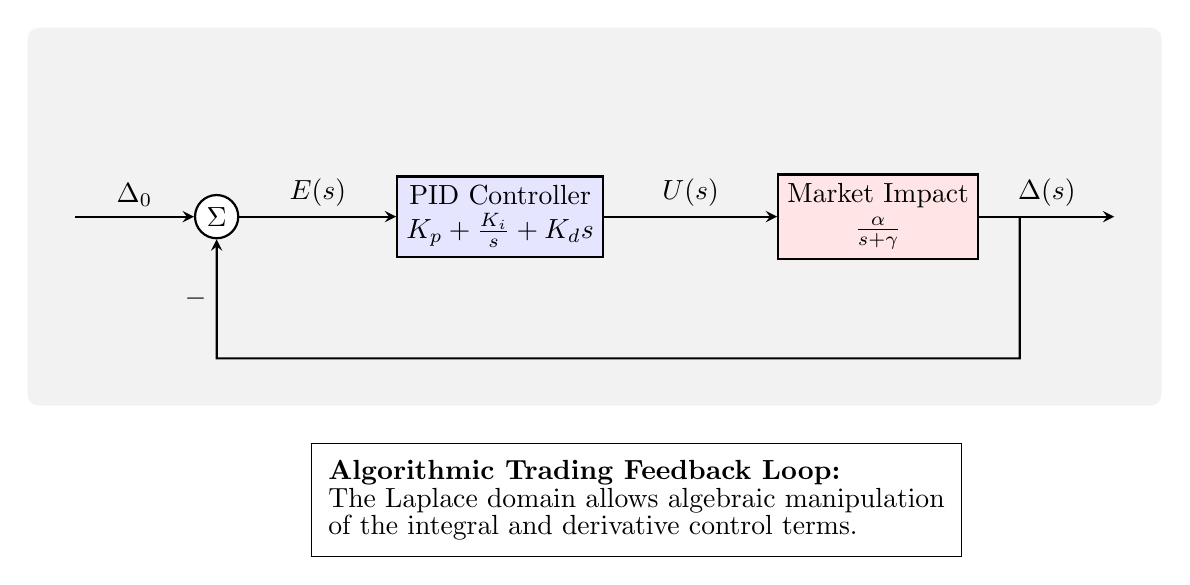
\begin{tikzpicture}[scale=1.2]
    % Background
    \fill[gray!10, rounded corners] (-1, -2) rectangle (11, 2);
    
    % Nodes
    \node[draw, thick, fill=white, circle, inner sep=2pt] (sum) at (1, 0) {$\Sigma$};
    \node[draw, thick, fill=blue!10, minimum width=2cm, minimum height=1cm, align=center] (pid) at (4, 0) {PID Controller \\ $K_p + \frac{K_i}{s} + K_d s$};
    \node[draw, thick, fill=red!10, minimum width=2cm, minimum height=1cm, align=center] (plant) at (8, 0) {Market Impact \\ $\frac{\alpha}{s + \gamma}$};
    
    % Arrows
    \draw[->, >=stealth, thick] (-0.5, 0) -- node[above] {$\Delta_0$} (sum.west);
    \draw[->, >=stealth, thick] (sum.east) -- node[above] {$E(s)$} (pid.west);
    \draw[->, >=stealth, thick] (pid.east) -- node[above] {$U(s)$} (plant.west);
    \draw[->, >=stealth, thick] (plant.east) -- node[above] {$\Delta(s)$} (10.5, 0);
    
    % Feedback loop
    \draw[->, >=stealth, thick] (9.5, 0) -- (9.5, -1.5) -- (1, -1.5) -- node[left] {$-$} (sum.south);
    
    % Legend
    \node[align=left, fill=white, draw=black, inner sep=6pt, anchor=west] at (2, -3) {
        \textbf{Algorithmic Trading Feedback Loop:} \\[-2pt]
        The Laplace domain allows algebraic manipulation \\[-2pt]
        of the integral and derivative control terms.
    };
\end{tikzpicture}
\end{center}

\section{Part 7: Common Variations and Untested Concepts}

\subsection{The Dirac Delta Function (Impulse Forcing)}
The provided homework covers step functions (Heaviside) but omits the Dirac delta function, $\delta(t-a)$, which models an instantaneous impulse (like a hammer strike or a sudden market shock).
\textbf{Concept:} $\Lap\{\delta(t-a)\} = e^{-as}$.
\textbf{Example:} Solve $y'' + y = \delta(t-\pi) ; \quad y(0)=0, y'(0)=0$.
\textit{Solution:} $s^2 Y + Y = e^{-\pi s} \implies Y(s) = e^{-\pi s} \frac{1}{s^2 + 1}$.
Using the second shifting theorem: $y(t) = \sin(t-\pi) u(t-\pi) = -\sin(t) u(t-\pi)$.

\subsection{Systems of Linear ODEs}
Laplace transforms are incredibly efficient for solving coupled systems of ODEs, which were not present in the homework.
\textbf{Example:} Solve $x' = 2x - y$ and $y' = x$, with $x(0)=1, y(0)=0$.
\textit{Solution:}
\begin{align*}
sX - 1 &= 2X - Y \implies (s-2)X + Y = 1 \\ \relax
sY &= X \implies X = sY
\end{align*}
Substitute $X$: $(s-2)(sY) + Y = 1 \implies (s^2 - 2s + 1)Y = 1 \implies Y = \frac{1}{(s-1)^2}$.
Thus $y(t) = te^t$. Since $x = y'$, $x(t) = e^t + te^t$.

\newpage
\section{Part 8: Advanced Diagnostic Testing: "Find the Flaw"}

Below are 5 problems with fully worked solutions. However, each solution contains a single, critical conceptual or algebraic flaw. \textbf{Your task as the grader is to identify the flaw, explain why it is wrong in one sentence, and provide the correct final answer.}

\subsection*{Flawed Problem 1}
\textbf{Problem:} Solve $y'' + 9y = 0 ; \quad y(0) = 2 , \quad y'(0) = 3$.
\textbf{Flawed Solution:}
\begin{align*}
\Lap\{y''\} + 9\Lap\{y\} &= 0 \\ \relax
(s^2 Y(s) - 2s) + 9Y(s) &= 0 \\ \relax
(s^2 + 9)Y(s) &= 2s \\ \relax
Y(s) &= \frac{2s}{s^2 + 9} \\ \relax
y(t) &= 2\cos 3t
\end{align*}

\subsection*{Flawed Problem 2}
\textbf{Problem:} Find the inverse Laplace transform of $Y(s) = \frac{s + 4}{s^2 + 4s + 13}$.
\textbf{Flawed Solution:}
\begin{align*}
Y(s) &= \frac{s + 4}{(s + 2)^2 + 9} \\ \relax
Y(s) &= \frac{s + 2}{(s + 2)^2 + 9} + \frac{2}{(s + 2)^2 + 9} \\ \relax
y(t) &= e^{-2t}\cos 3t + 2e^{-2t}\sin 3t
\end{align*}

\subsection*{Flawed Problem 3}
\textbf{Problem:} Solve $ty'' + y' = 0 ; \quad y(0) = 1 , \quad y'(0) = 0$.
\textbf{Flawed Solution:}
\begin{align*}
\Lap\{ty''\} + \Lap\{y'\} &= 0 \\ \relax
-\frac{d}{ds}[s^2 Y(s) - s(1) - 0] + [sY(s) - 1] &= 0 \\ \relax
-[2sY(s) + s^2 Y'(s) - 1] + sY(s) - 1 &= 0 \\ \relax
-s^2 Y'(s) - sY(s) &= 0 \\ \relax
Y'(s) + \frac{1}{s}Y(s) &= 0 \\ \relax
Y(s) &= \frac{C}{s} \implies y(t) = C
\end{align*}
Since $y(0) = 1$, $C = 1$. Final answer: $y(t) = 1$.

\subsection*{Flawed Problem 4}
\textbf{Problem:} Solve $y'' - y = e^t ; \quad y(0) = 0 , \quad y'(0) = 0$.
\textbf{Flawed Solution:}
\begin{align*}
s^2 Y(s) - Y(s) &= \frac{1}{s - 1} \\ \relax
(s^2 - 1)Y(s) &= \frac{1}{s - 1} \\ \relax
Y(s) &= \frac{1}{(s - 1)^2(s + 1)} = \frac{A}{s - 1} + \frac{B}{(s - 1)^2} + \frac{C}{s + 1}
\end{align*}
Using cover-up, $B = 1/2$ and $C = 1/4$.
$Y(s) = \frac{A}{s - 1} + \frac{1/2}{(s - 1)^2} + \frac{1/4}{s + 1}$.
$y(t) = Ae^t + \frac{1}{2}te^t + \frac{1}{4}e^{-t}$.

\subsection*{Flawed Problem 5}
\textbf{Problem:} Solve $y'' + y = u(t - 2) ; \quad y(0) = 0 , \quad y'(0) = 0$.
\textbf{Flawed Solution:}
\begin{align*}
s^2 Y(s) + Y(s) &= \frac{e^{-2s}}{s} \\ \relax
Y(s) &= e^{-2s} \frac{1}{s(s^2 + 1)} = e^{-2s} \left( \frac{1}{s} - \frac{s}{s^2 + 1} \right) \\ \relax
y(t) &= (1 - \cos t) u(t - 2)
\end{align*}

\end{document}